\usetikzlibrary{shapes}
\usetikzlibrary{decorations.shapes}

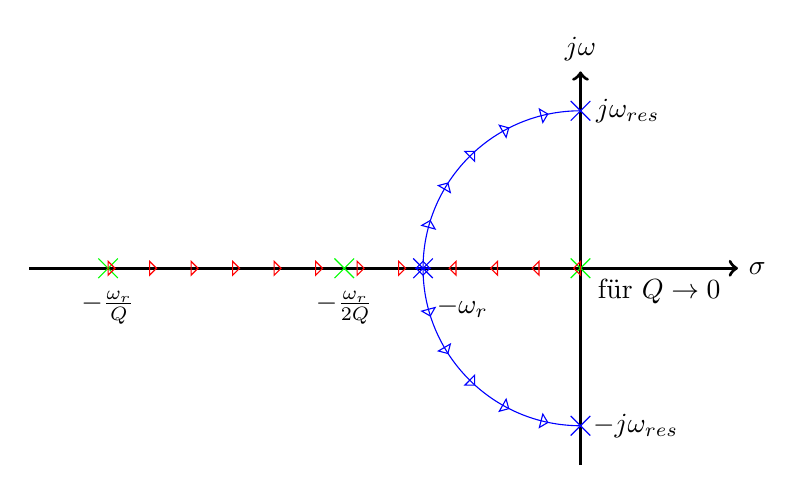
\begin{tikzpicture}
% Koordinatensystem
\begin{scope}[->, very thick]
	\draw (-7,0) -- (2,0) node[right] {$\sigma$};
	\draw (0,-2.5) -- (0,2.5) node[above] {$j\omega$};
\end{scope}

% Nullstellen
\node[cross out, draw=green] at (0,0) {} ;
\node at(1,-0.3) {für $Q \rightarrow 0$};
\node[cross out, draw=green] at (-6,0) {};
\node at(-6, -0.5) {$-\frac{\omega_r}{Q}$};
\node[cross out, draw=green] at (-3,0) {};
\node at(-3, -0.5) {$-\frac{\omega_r}{2Q}$};

% Rote Pfeile
\begin{scope}[draw=red, decoration={triangles, shape height=5, segment length=15}]
	\draw[decorate] (0,0) -- (-2,0);
	\draw[decorate] (-6,0) -- (-2,0);
\end{scope}

% Blauer Halbkreis mit Nullstelle und so.
\begin{scope}[draw=blue]
	\node[cross out, draw] at (-2,0) {};
	\node at(-1.5, -0.5) {$-\omega_r$};
	\draw (-2,0) arc (180:90:2);
	\draw (-2,0) arc (180:270:2);
	\node[cross out, draw] at (0,2) {};
	\node at (0.6, 2) {$j\omega_{res}$};
	\node[cross out, draw] at (0,-2) {};
	\node at (0.7, -2) {$-j\omega_{res}$};
\end{scope}

% Blaue Dreieckli
\begin{scope}[draw=blue, decoration={triangles, shape height=5, segment length=15}]
	\draw[decorate] (-2,0) arc (180:90:2);
	\draw[decorate] (-2,0) arc (180:270:2);
\end{scope}
\end{tikzpicture}